\documentclass[12pt]{article}
\usepackage[utf8]{inputenc}
\usepackage[T1]{fontenc}
\usepackage[spanish]{babel}
\usepackage{graphicx}
\usepackage{caption}
\usepackage{subcaption}
\usepackage{geometry}
\geometry{a4paper, margin=2.5cm}
\usepackage{booktabs}
\usepackage{hyperref}
\usepackage{amsmath}

\title{Análisis de Predictibilidad y Contornos de Parámetros}
\author{Modelo SBMe / Forecasting}
\date{\today}

\begin{document}

\maketitle

\section{Procedimiento de Calibración y Visualización}

El análisis se basa en un modelo sintético de dispersión epidémica generado con un SBM (Stochastic Block Model) y un modelo surrogate que estima la evolución de la fracción infectada. El objetivo es evaluar cómo cambia la incertidumbre del ajuste de parámetros y la predictibilidad en tres escenarios de origen temporal:

\begin{itemize}
  \item \textbf{Pre-peak:} origen 14 días antes del pico (\texttt{t\_peak - 14}).
  \item \textbf{At-peak:} origen en el día del pico (\texttt{t\_peak}).
  \item \textbf{Post-peak:} origen 14 días después del pico (\texttt{t\_peak + 14}).
\end{itemize}

En cada escenario el procedimiento consiste en:

\begin{enumerate}
  \item Generar la curva objetivo sintética usando \texttt{generate\_sbm\_target.py}.
  \item Ajustar el modelo al subconjunto de datos conocidos hasta el corte temporal \texttt{t\_cut}.
  \item Evaluar múltiples candidatos en el espacio de parámetros \((\beta_{network},\; \beta_{household},\; \delta,\; \mu)\).
  \item Seleccionar los mejores ajustes según error de calibración y construir el conjunto \texttt{TOP\_K} de parámetros aceptados.
  \item Generar trayectorias predictivas con los parámetros aceptados y estimar la mediana predictiva junto con los percentiles 10 y 90.
  \item Visualizar la densidad de parámetros con diagramas de contorno KDE y evaluar la banda de incertidumbre de la predicción.
\end{enumerate}

\section{Figura de Contornos de Confianza}

La figura de la Sección~\ref{fig:contornos} muestra las densidades de parámetros para cada escenario. Los contornos se obtienen a partir de los mejores ajustes y reflejan la distribución posterior aproximada de los parámetros.

\begin{figure}[htbp]
  \centering
  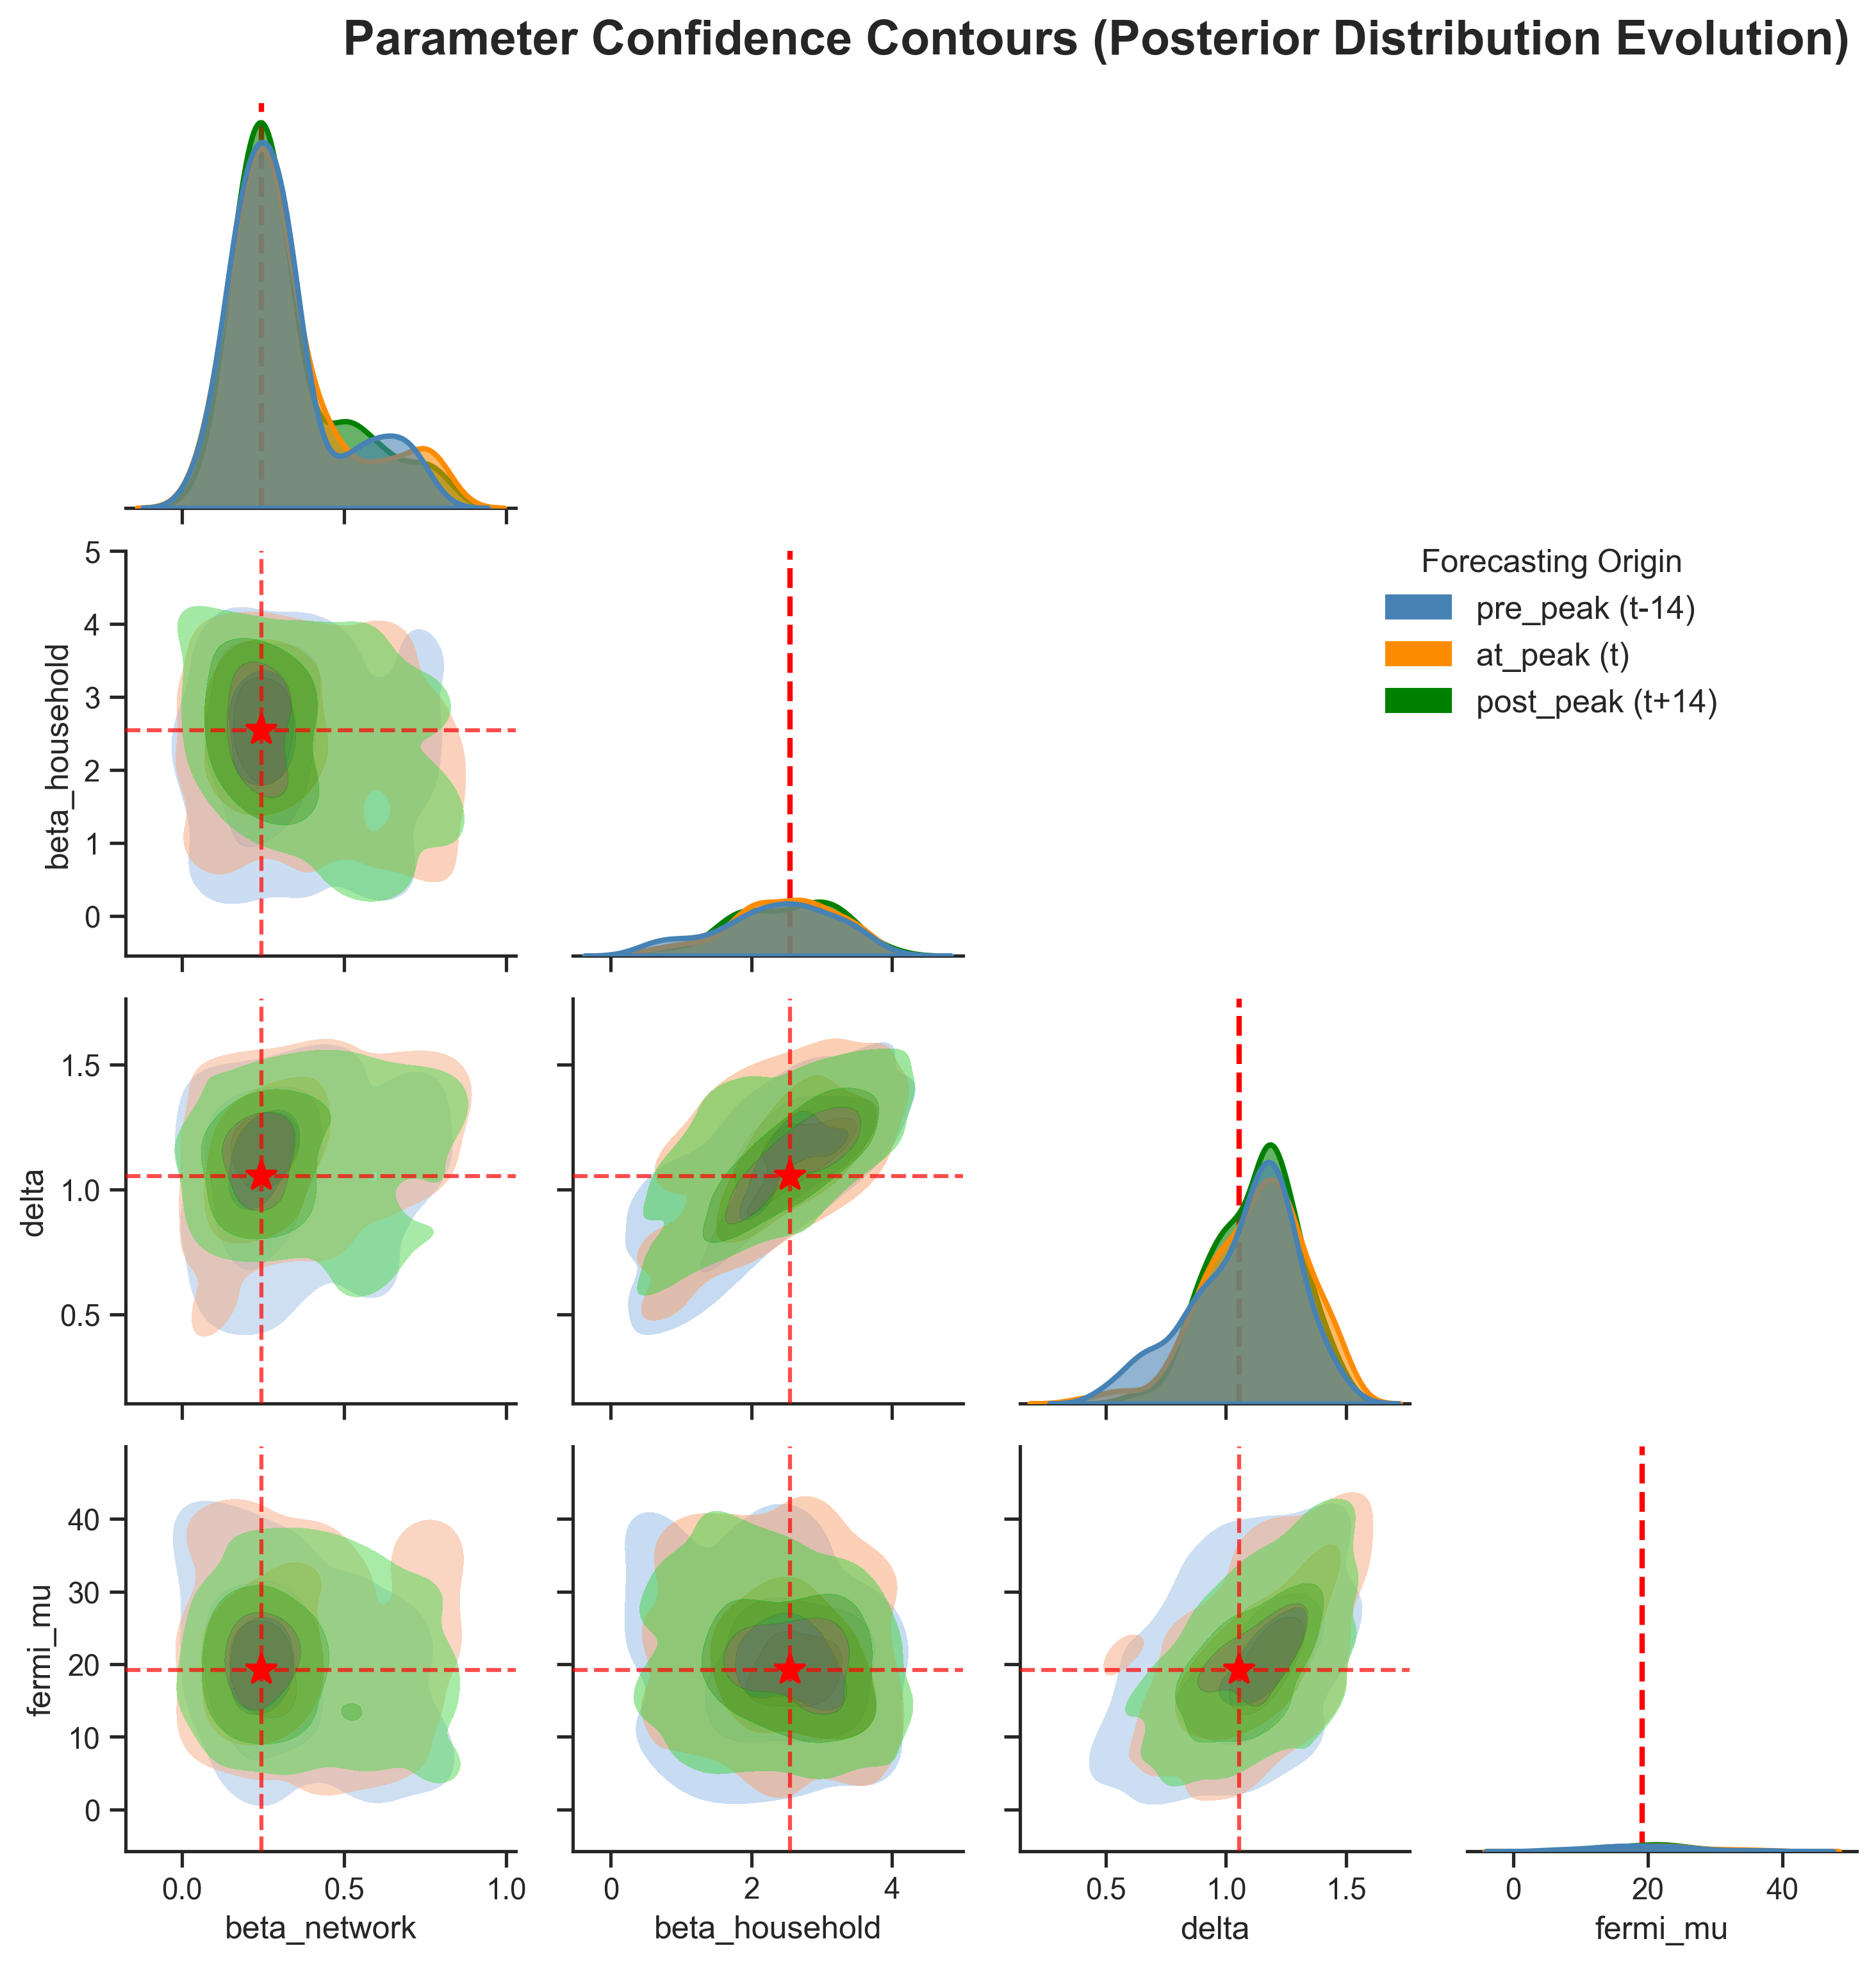
\includegraphics[width=0.95\textwidth]{output/parameter_confidence_contours.png}
  \caption{Contornos de confianza de los parámetros. Cada color corresponde a un horizonte de calibración diferente: pre-peak, at-peak y post-peak.}
  \label{fig:contornos}
\end{figure}

\section{Criterio de Horizonte de Predictibilidad}

El horizonte de predictibilidad se define a partir del ancho de la banda percentil 10--90. Para cada día futuro \(h\), la incertidumbre puntual se mide como:

\[
  W(h) = P_{90}(h) - P_{10}(h).
\]

Este ancho no se normaliza por la mediana local de ese mismo día, porque esa elección penaliza artificialmente la cola descendente de la epidemia cuando la fracción infectada es pequeña. En su lugar, se usa una referencia global de la curva predicha completa. Para cada escenario se reconstruyen las trayectorias completas predichas en el intervalo \(t=0,\ldots,100\) con el conjunto de parámetros aceptados, se calcula su mediana temporal completa y se toma su máximo:

\[
  I^{pred}_{max} = \max_{t \in [0,100]} \widetilde{I}^{pred}(t).
\]

La razón de incertidumbre global queda entonces:

\[
  R(h) = \frac{P_{90}(h) - P_{10}(h)}{I^{pred}_{max}}.
\]

El límite de predictibilidad \(H_{max}\) corresponde al primer día futuro en el que esta razón supera el umbral seleccionado:

\[
  H_{max} = \min \{h : R(h) > 0.75 \}.
\]

Si la razón no supera el umbral durante el horizonte disponible, se considera que toda la ventana restante es predecible. Con este criterio, el error usado es siempre el ancho de percentiles 10--90 en cada punto del pronóstico, pero expresado de forma relativa respecto a una escala global común de la predicción completa.

\section{Figura de Horizonte de Predictibilidad}

La figura de la Sección~\ref{fig:predictabilidad} muestra la curva objetivo, la historia conocida, la mediana predictiva, la banda de incertidumbre 10\%--90\%, y el límite de predictibilidad definido mediante el criterio global anterior. La línea naranja marca el primer punto donde \(R(h)\) supera el umbral de 0.75.

\begin{figure}[htbp]
  \centering
  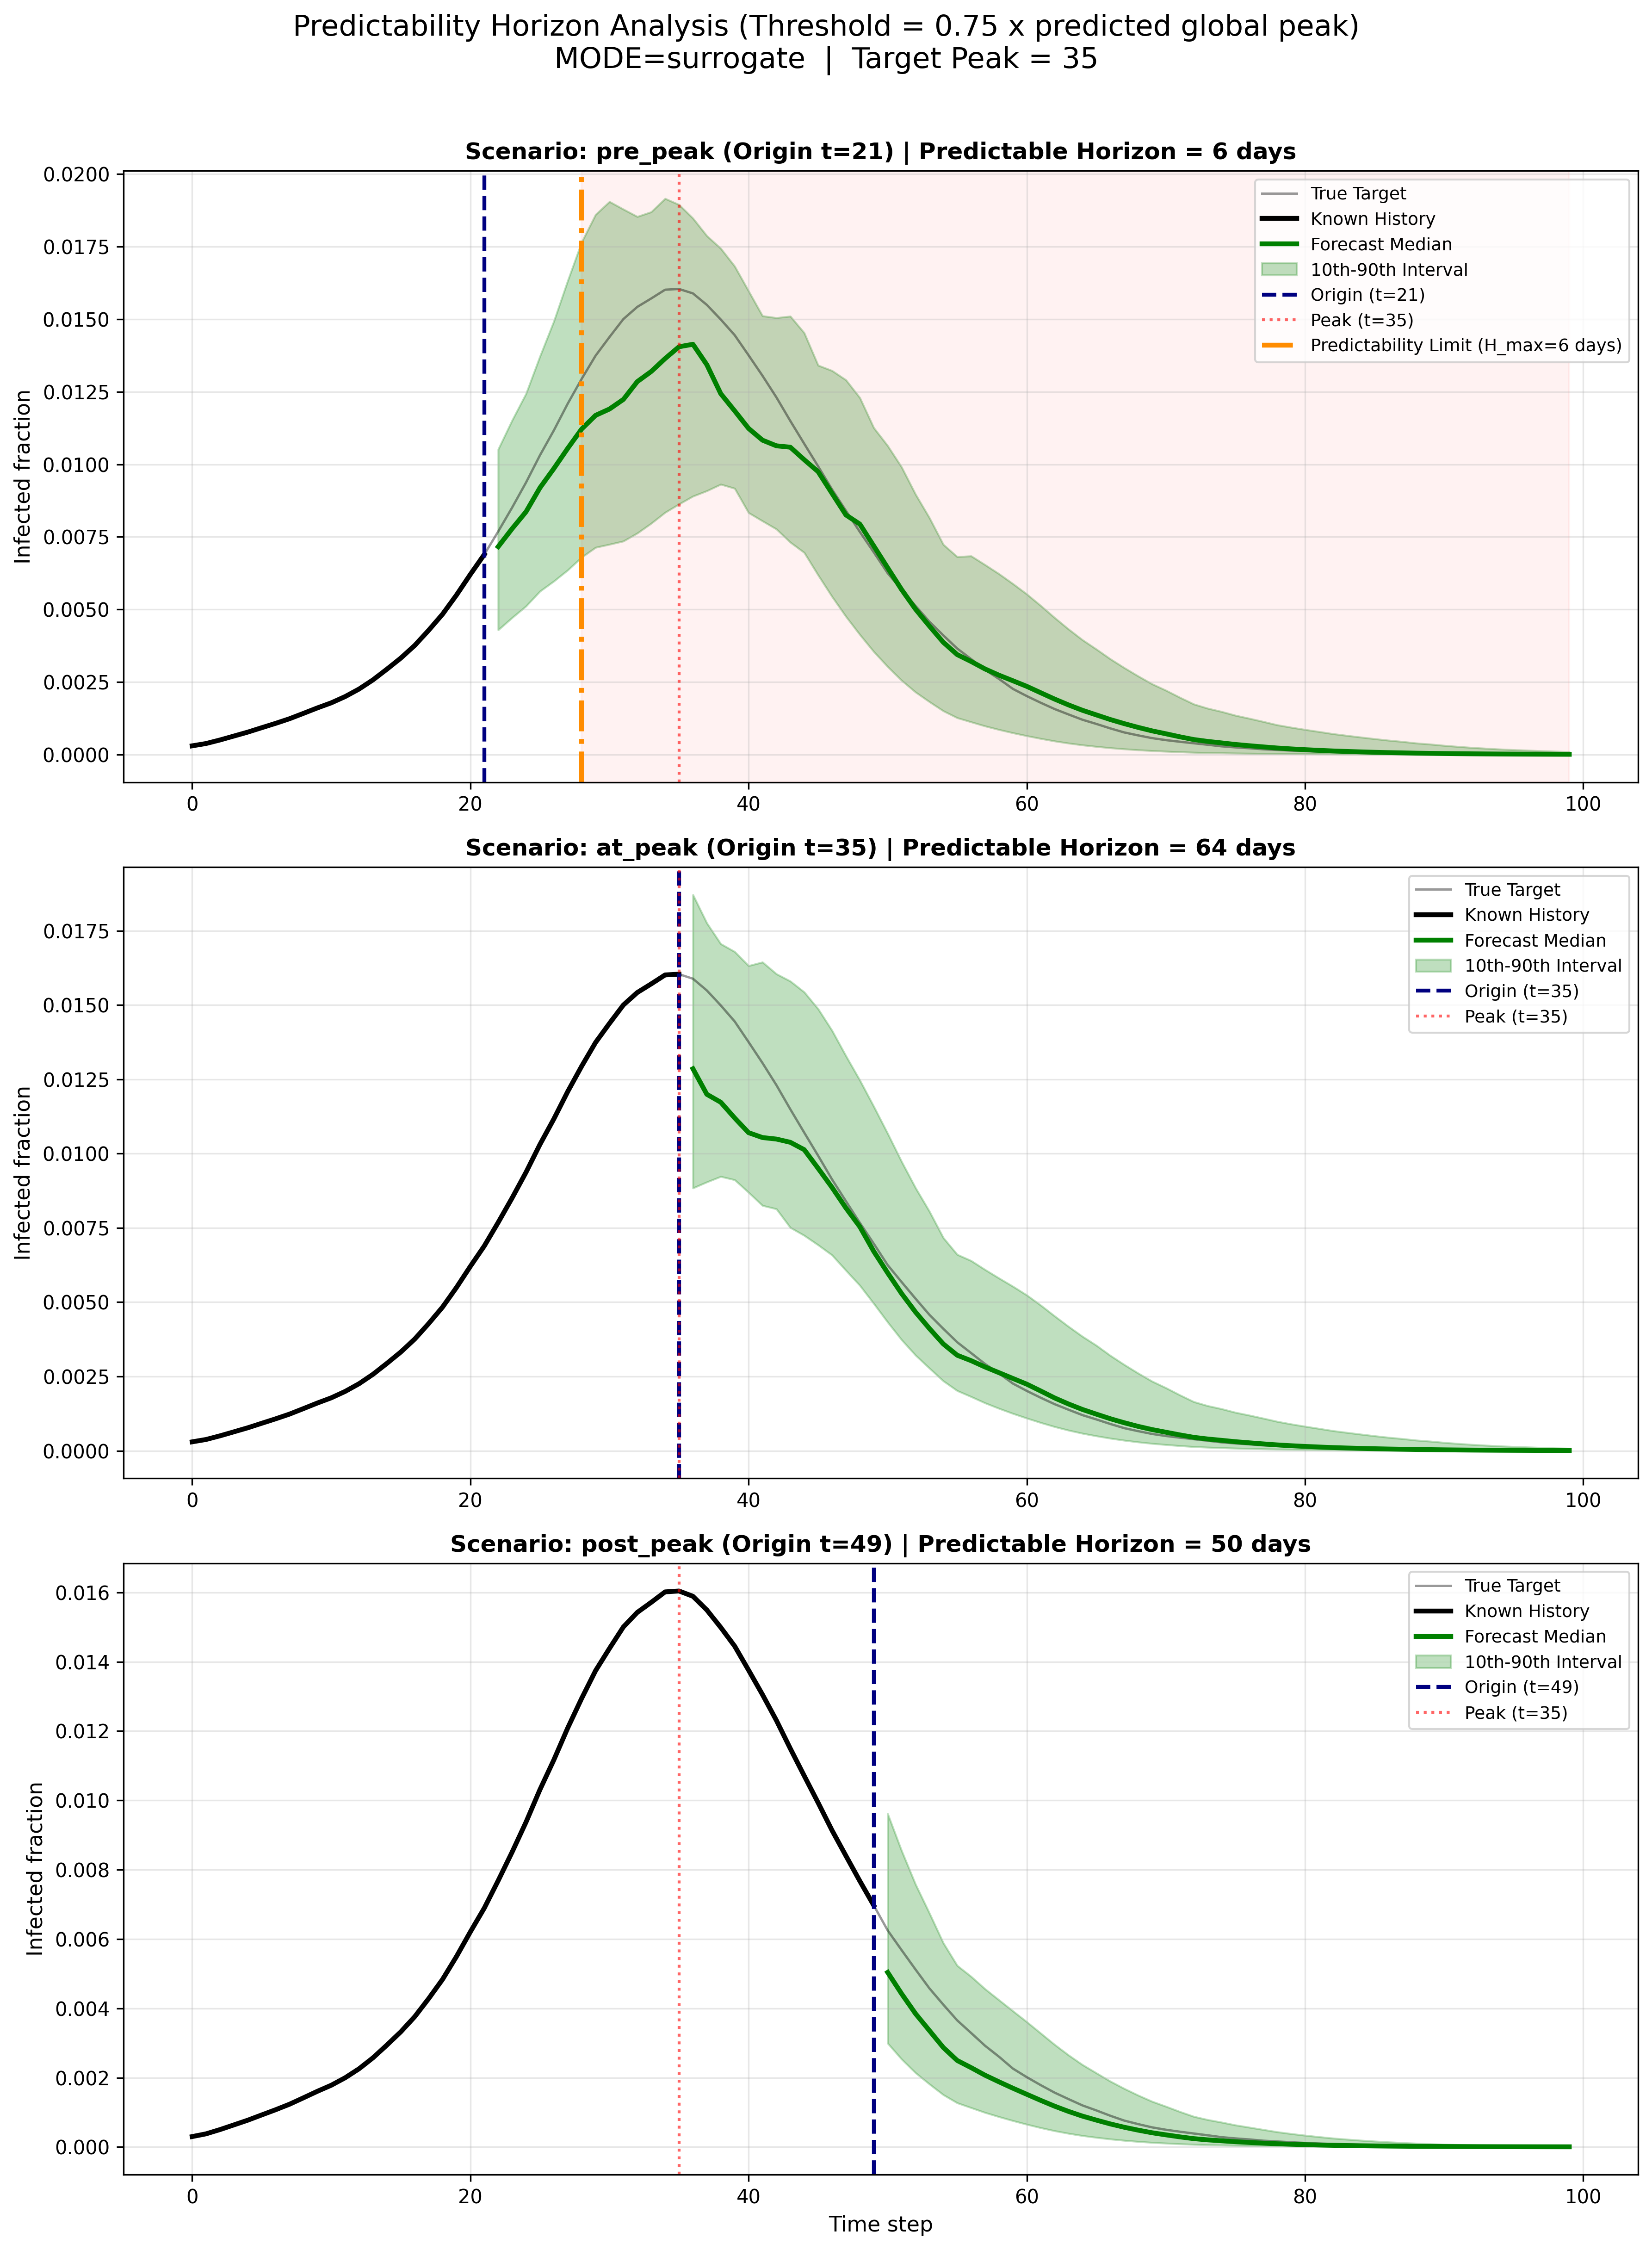
\includegraphics[width=0.95\textwidth]{output/predictability_horizon.png}
  \caption{Análisis de horizonte de predictibilidad para los tres escenarios de origen. La región sombreada indica el intervalo de incertidumbre, y la línea naranja marca el punto donde la predicción deja de ser confiable.}
  \label{fig:predictabilidad}
\end{figure}

\section{Interpretación}

Del análisis se extrae que el ajuste de parámetros y la predictibilidad varían significativamente según la información disponible en el origen de la predicción. Al normalizar la incertidumbre por el pico global de la curva predicha completa, los escenarios se comparan en una escala más estable que la mediana local. Esto evita clasificar como no predecible una fase post-pico únicamente porque el valor infectado local ya es pequeño.

Con el umbral \(0.75\), el escenario pre-peak mantiene un horizonte de predictibilidad corto, porque todavía existe dispersión importante sobre la forma posterior de la epidemia. En cambio, los escenarios at-peak y post-peak conservan horizontes largos, ya que la historia observada contiene suficiente información sobre el pico y la fase descendente para reducir la incertidumbre relativa de la banda 10--90.

\end{document}
